\documentclass[notes,11pt, aspectratio=169]{beamer}
\usepackage[default]{lato}


\newenvironment{transitionframe}{
  \setbeamercolor{background canvas}{bg=yellow}
  \begin{frame}}{
    \end{frame}
}


\setbeamercolor{frametitle}{fg=blue}
\setbeamercolor{title}{fg=black}
\setbeamertemplate{footline}[frame number]
\setbeamertemplate{navigation symbols}{} 
\setbeamertemplate{itemize items}{-}
\setbeamercolor{itemize item}{fg=blue}
\setbeamercolor{itemize subitem}{fg=blue}
\setbeamercolor{enumerate item}{fg=blue}
\setbeamercolor{enumerate subitem}{fg=blue}
\setbeamercolor{button}{bg=MyBackground,fg=blue,}


% If you like road maps, rather than having clutter at the top, have a roadmap show up at the end of each section 
% (and after your introduction)
% Uncomment this is if you want the roadmap!
% \AtBeginSection[]
% {
%    \begin{frame}
%        \frametitle{Roadmap of Talk}
%        \tableofcontents[currentsection]
%    \end{frame}
% }
\setbeamercolor{section in toc}{fg=blue}
\setbeamercolor{subsection in toc}{fg=red}
\setbeamersize{text margin left=1em,text margin right=1em} 

\newenvironment{wideitemize}{\itemize\addtolength{\itemsep}{10pt}}{\enditemize}


\AtBeginSection[]{
  \begin{frame}
  \vfill
  \centering
  \begin{beamercolorbox}[sep=8pt,center,shadow=true,rounded=true]{title}
    \usebeamerfont{title}\insertsectionhead\par%
  \end{beamercolorbox}
  \vfill
  \end{frame}
}

%\setbeamertemplate{caption}[numbered]
\usepackage{adjustbox}
\usepackage{threeparttable}
\usepackage{graphicx}
\usepackage{multicol}
\usepackage{natbib}
\usepackage{float}
\usepackage{url}
\usepackage{hyperref}
\usepackage{color}
\usepackage{tabls, calc}
\usepackage[tableposition=top]{caption}
\usepackage{ifthen}
\usepackage{setspace}
\usepackage{booktabs}
\usepackage[english]{babel}
\usepackage[latin1]{inputenc}
\usepackage{caption}
\usepackage{subfigure}	
%\usepackage{custom}
\usepackage{tikz}
\usepackage{array}
\usepackage{dcolumn}
\usepackage{multirow}
\usepackage{markdown}
\usepackage{siunitx}
\usepackage{tfrupee}
%\usepackage[table]{xcolor}
%\usepackage{xcolor}
\usepackage{colortbl}
\usepackage{tcolorbox}

\tcbset{width=0.9\textwidth,boxrule=0pt,colback=red,arc=0pt,auto outer arc,left=0pt,right=0pt,boxsep=5pt}


%%%%%%%%%%%%%%%%%%%%%%%%%%%%%5
\usepackage{listings}
\definecolor{codegreen}{rgb}{0,0.6,0}
\definecolor{codegray}{rgb}{0.5,0.5,0.5}
\definecolor{codepurple}{rgb}{0.58,0,0.82}
\definecolor{backcolour}{rgb}{0.95,0.95,0.92}

\lstdefinestyle{mystyle}{
    backgroundcolor=\color{backcolour},   
    commentstyle=\color{codegreen},
    keywordstyle=\color{magenta},
    numberstyle=\tiny\color{codegray},
    stringstyle=\color{codepurple},
    basicstyle=\ttfamily\footnotesize,
    breakatwhitespace=false,         
    breaklines=true,                 
    captionpos=b,                    
    keepspaces=true,                 
    numbers=left,                    
    numbersep=5pt,                  
    showspaces=false,                
    showstringspaces=false,
    showtabs=false,                  
    tabsize=2
}

\lstset{style=mystyle}


%%%%%%%%%%%%%%%%%%%%%%%%%%%%
\newcommand{\Note}[1]{
\rule{2.5cm}{0.25pt} \\ \textit{\footnotesize{\textcolor{rubineRed}{Note:} \textcolor{darkerGray}{#1}}}}

\newcommand{\formula}[1]{
\begin{beamerboxesrounded}[shadow = false, lower = formula body]{}
#1
\end{beamerboxesrounded}
}

\setbeamercolor{prac ques body}{fg=oiB}

\newcommand{\pq}[1]{
\begin{beamerboxesrounded}[shadow = false, lower = prac ques body]{}
#1
\end{beamerboxesrounded}
}



%%%%%%%%%%%%%%%%%%%%%%%%%%%%%%%
\newcommand{\hl}[1]{\textit{\textcolor{hlblue}{#1}}}
\newcommand{\hlGr}[1]{\textit{\textcolor{lightGreen}{#1}}}
\newcommand{\mathhl}[1]{\textcolor{hlblue}{\ensuremath{#1}}}


%%%Define Colors Here
\definecolor{applegreen}{rgb}{0.55, 0.71, 0.0}
\definecolor{ao(english)}{rgb}{0.0, 0.5, 0.0}
\definecolor{pink}{rgb}{0.858, 0.188, 0.478}
\definecolor{purple}{HTML}{6A5ACD}
\definecolor{orange}{HTML}{FFA500}
\definecolor{denim}{rgb}{0.08, 0.38, 0.74}
\definecolor{seagreen}{rgb}{0.13, 0.7, 0.67}
\definecolor{tangerine}{rgb}{0.95, 0.52, 0.0}
\definecolor{textboxgreen}{rgb}{0.67, 0.88, 0.69}
\definecolor{textboxred}{HTML}{BF616A}
\definecolor{redPink}{HTML}{e64173}
\definecolor{turquoise}{HTML}{20B2AA}
\definecolor{backcolour}{rgb}{0.95,0.95,0.92}
\xdefinecolor{oiB}{rgb}{0.22,0.52,0.72}
\definecolor{oiG}{rgb}{.298,.447,.114}
\xdefinecolor{hlblue}{rgb}{0.051,0.65,1}
\xdefinecolor{gray}{rgb}{0.5, 0.5, 0.5}
\xdefinecolor{darkGray}{rgb}{0.3, 0.3, 0.3}
\xdefinecolor{darkerGray}{rgb}{0.2, 0.2, 0.2}
\xdefinecolor{rubineRed}{rgb}{0.89,0,0.30}
\xdefinecolor{irishGreen}{rgb}{0,0.60,0}	
\definecolor{lightGreen}{rgb}{0.387,0.581,0.148} 
\setbeamercolor{frametitle}{fg=denim}

%$%%%%%%%%%%%%%%%%%%%%%%%%%%%%%%%%%
\newcommand{\dq}[1]{
\begin{beamerboxesrounded}[shadow = false, lower = disc ques body]{}
#1
\end{beamerboxesrounded}
}

% solnMult: solutions for practice questions

\newcommand{\solnMult}[1]{
\item[] \vspace{-0.59cm}
\only<1>{\item #1}
\soln{\only<2->{\item \orange{#1}}}
}

% removepagenumbers
\newcommand{\removepagenumbers}{% 
  \setbeamertemplate{footline}{}
}

\newcommand{\soln}[1]{\textit{#1}}
\newcommand{\solnGr}[1]{#1}


%%%%%%%%%%%%%%%%
\usepackage{geometry}
\usepackage{graphicx}
\usepackage{amssymb}
%\usepackage{cancel}
\usepackage{epstopdf}
\usepackage{amsmath}  	% this permits text in eqnarray among other benefits
\usepackage{url}		% produces hyperlinks
\usepackage{hyperref}	% allows for color usage in tables
\usepackage[english]{babel}
\usepackage[latin1]{inputenc}
\usepackage{colortbl}	% allows for color usage in tables
\usepackage{multirow}	% allows for rows that span multiple rows in tables
\usepackage{color}		% this package has a variety of color options
\usepackage{pgf}
\usepackage{calc}
\usepackage{ulem}
\usepackage{multicol}
\usepackage{textcomp}
%\usepackage{txfonts}
\usepackage{listings}
\usepackage{tikz}
\usepackage{array}
\usepackage{wasysym}
\usepackage{fancyvrb}
%%%%%%%%%%%%%%%%

%%%%%%%%%%%%%%%%
% Custom commands
%%%%%%%%%%%%%%%%

% degree
\newcommand{\degree}{\ensuremath{^\circ}}


% cite
\newcommand{\ct}[1]{
\vfill
{\tiny #1}}


% Remember
\newcommand{\Remember}[1]{\textit{\scriptsize{\textcolor{orange}{Remember:} #1}}}

% expected counts
\newcommand{\ex}[1]{\textit{\textcolor{blue}{#1}}}

% red
\newcommand{\red}[1]{\textit{\textcolor{rubineRed}{#1}}}

% pink
\newcommand{\pink}[1]{\textit{\textcolor{rubineRed!90!white!50}{#1}}}

% green
\newcommand{\green}[1]{\textit{\textcolor{irishGreen}{#1}}}

% orange
\newcommand{\orange}[1]{\textit{\textcolor{orange}{#1}}}

% links: webURL, webLin, appLink
\newcommand{\webURL}[1]{\urlstyle{same}{ \textit{\textcolor{darkGray}{\url{#1}}}}}
\newcommand{\webLink}[2]{\href{#1}{\textcolor{darkGray}{{#2}}}}
\newcommand{\appLink}[2]{\href{#1}{\textcolor{white}{{#2}}}}

% mail
\newcommand{\mail}[1]{\href{mailto:#1}{\textit{\textcolor{darkGray}{#1}}}}


% two col: two columns
\newenvironment{twocol}[4]{
\begin{columns}[c]
\column{#1\textwidth}
#3
\column{#2\textwidth}
#4
\end{columns}
}




% slot (for probability calculations)
\newenvironment{slot}[2]{
\begin{array}{c} 
\underline{#1} \\ 
#2
\end{array}
}

% pr: left and right parentheses
\newcommand{\pr}[1]{
\left( #1 \right)
}


% cancel
\newcommand{\cancel}[1]{%
    \tikz[baseline=(tocancel.base)]{
        \node[inner sep=0pt,outer sep=0pt] (tocancel) {#1};
        \draw[red, line width=0.5mm] (tocancel.south west) -- (tocancel.north east);
    }%
}


%%%%%%%%%%%%%%%%
% Custom boxes
%%%%%%%%%%%%%%%%

% app: application exercise

\setbeamercolor{app body}{fg=oiG}

\newcommand{\app}[1]{
\begin{beamerboxesrounded}[shadow = false, lower = app body]{}
#1
\end{beamerboxesrounded}
}


%%%%%%%%%%%%%%%%
% Change margin
%%%%%%%%%%%%%%%%

\newenvironment{changemargin}[2]{%
\begin{list}{}{%
\setlength{\topsep}{0pt}%
\setlength{\leftmargin}{#1}%
\setlength{\rightmargin}{#2}%
\setlength{\listparindent}{\parindent}%
\setlength{\itemindent}{\parindent}%
\setlength{\parsep}{\parskip}%
}%
\item}{\end{list}}

%%%%%%%%%%%%%%%%
% Footnote
%%%%%%%%%%%%%%%%

\long\def\symbolfootnote[#1]#2{\begingroup%
\def\thefootnote{\fnsymbol{footnote}}\footnote[#1]{#2}\endgroup}

%%%%%%%%%%%%%%%%
% Commands from the book
%%%%%%%%%%%%%%%%

\newenvironment{data}[1]{\texttt{#1}}{}
\newenvironment{var}[1]{\texttt{#1}}{}
\newenvironment{resp}[1]{\texttt{#1}}{}

%%%%%%%%%%%%%%%%
% Graphics
%%%%%%%%%%%%%%%%

\DeclareGraphicsRule{.tif}{png}{.png}{`convert #1 `dirname #1`/`basename #1 .tif`.png}



%----------------------------------------------------------------------------------------
%	TITLE PAGE
%----------------------------------------------------------------------------------------
\title[DAR]{Data Analytics with R}  % The short title appears at the bottom of 
\author{Sumit Mishra} % Your name
\institute[IFMR] % Your institution as it will appear on the bottom of every slide, may be shorthand to save space
{
Institute for Financial Management and Research, Sri City \\ % Your institution for the title page
\medskip
\medskip
\textbf{Probability} % Your email address
}
\date{11 November 2020} % Date, can be changed to a custom date

%%%%%%%%%%%%%%%%%%%%%%%%%%%%%%%%%%%%
% Begin document
%%%%%%%%%%%%%%%%%%%%%%%%%%%%%%%%%%%%
\begin{document}


%%%%%%%%%%%%%%%%%%%%%%%%%%%%%%%%%%%%
% Title page
%%%%%%%%%%%%%%%%%%%%%%%%%%%%%%%%%%%%

{
\addtocounter{framenumber}{-1} 
{\removepagenumbers 
%\usebackgroundtemplate{\includegraphics[width=\paperwidth]{../OpenIntro_Grid_4_3-01.jpg}}
\begin{frame}

%\hfill \includegraphics[width=20mm]{../oiLogo_highres}

\titlepage

\end{frame}
}
}

%%%%%%%%%%%%%%%%%%%%%%%%%%%%%%%%%%%%

\section{Defining probability}

%%%%%%%%%%%%%%%%%%%%%%%%%%%%%%%%%%%%

\subsection{Probability}

%%%%%%%%%%%%%%%%%%%%%%%%%%%%%%%%%%%%

%%%%%%%%%%%%%%%%%%%%%%%%%%%%%%%%%%%%%%%%%%
\begin{frame}
\frametitle{Random processes}

\begin{columns}
\column{0.5\textwidth}
\begin{itemize}

\item A \hl{random process} is a situation in which we know what outcomes could happen, but we don't know which particular outcome will happen.

\item Examples: coin tosses, die rolls, iTunes shuffle, whether the stock market goes up or down tomorrow, etc.

\item It can be helpful to model a process as random even if it is not truly random.

\end{itemize}
\column{0.5\textwidth}
\begin{center}
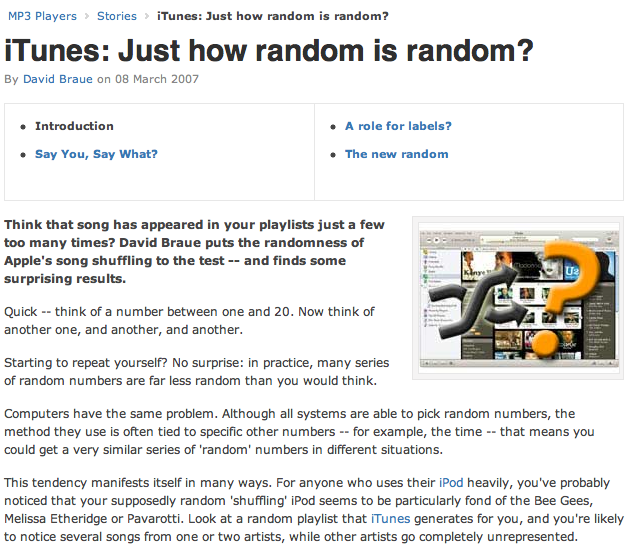
\includegraphics[width=\textwidth]{3-1_define_probability/figures/iTunes}
\end{center}
\end{columns}
\ct{ \webURL{http://www.cnet.com.au/itunes-just-how-random-is-random-339274094.htm}}


\end{frame}


%%%%%%%%%%%%%%%%%%%%%%%%%%%%%%%%%%%%%%%%%%%

%%%%%%%%%%%%%%%%%%%%%%%%%%%%%%%%%%%%

\begin{frame}
\frametitle{Probability}

\begin{itemize}

\item There are several possible interpretations of probability but they (almost) completely agree on the mathematical rules probability must follow.
\begin{itemize}
\item $P(A)$ = Probability of event A 
\item $0 \le P(A) \le 1$
\end{itemize}

\pause

\item \hl{Frequentist interpretation:} 
\begin{itemize}
\item The probability of an outcome is the proportion of times the outcome would occur if we observed the random process an infinite number of times.
\end{itemize}

\pause

\item \hl{Bayesian interpretation:} 
\begin{itemize}
\item  A Bayesian interprets probability as a subjective degree of belief: For the same event, two separate people could have different viewpoints and so assign different probabilities.
\item Largely popularized by revolutionary advance in computational technology and methods during the last twenty years.
\end{itemize}

\end{itemize}

\end{frame}

%%%%%%%%%%%%%%%%%%%%%%%%%%%%%%%%%%%%

\begin{frame}
\frametitle{Practice}

\pq{Which of the following events would you be most surprised by?}

\begin{enumerate}[(a)]
\item exactly 3 heads in 10 coin flips
\item exactly 3 heads in 100 coin flips
\solnMult{exactly 3 heads in 1000 coin flips}
\end{enumerate}

\end{frame}

%%%%%%%%%%%%%%%%%%%%%%%%%%%%%%%%%%%%

\begin{frame}
\frametitle{Law of large numbers}

\hl{Law of large numbers} states that as more observations are collected, the proportion of occurrences with a particular outcome, \mathhl{\hat{p}_n}, converges to the probability of that outcome, \mathhl{p}.

\end{frame}

%%%%%%%%%%%%%%%%%%%%%%%%%%%%%%%%%%%%

\begin{frame}
\frametitle{Law of large numbers (cont.)}

\dq{When tossing a \textit{fair} coin, if heads comes up on each of the first 10 tosses, what do you think the chance is that another head will come up on the next toss? 0.5, less than 0.5, or more than 0.5?}

\[ \underline{H} \hspace{1mm} \underline{H} \hspace{1mm} \underline{H} \hspace{1mm} \underline{H} \hspace{1mm} \underline{H} \hspace{1mm} \underline{H} \hspace{1mm} \underline{H} \hspace{1mm} \underline{H} \hspace{1mm} \underline{H} \hspace{1mm} \underline{H} \hspace{1mm} \underline{?} \]

\begin{itemize}
\item<2-> The probability is still 0.5, or there is still a 50\% chance that another head will come up on the next toss.
\[ P(H \text{ on 11}^{th} \text{ toss}) = P(T \text{ on 11}^{th} \text{ toss}) = 0.5 \]
\item<3-> The coin is not ``due" for a tail.
\item<4-> The common misunderstanding of the LLN is that random processes are supposed to compensate for whatever happened in the past; this is just not true and is also called \hl{gambler's fallacy} (or \hl{law of averages}).
\end{itemize}

\end{frame}

%%%%%%%%%%%%%%%%%%%%%%%%%%%%%%%%%%%%

\subsection{Disjoint or mutually exclusive outcomes}

%%%%%%%%%%%%%%%%%%%%%%%%%%%%%%%%%%%%

\begin{frame}
\frametitle{Disjoint and non-disjoint outcomes}

\hl{Disjoint (mutually exclusive) outcomes:} Cannot happen at the same time.
\begin{itemize}
\item The outcome of a single coin toss cannot be a head and a tail.
\item A student both cannot fail and pass a class.
\item A single card drawn from a deck cannot be an ace and a queen.
\end{itemize}

\pause

\hl{Non-disjoint outcomes:} Can happen at the same time.
\begin{itemize}
\item A student can get an A in Stats and A in Econ in the same semester.
\end{itemize}

\end{frame}

%%%%%%%%%%%%%%%%%%%%%%%%%%%%%%%%%%%%

\begin{frame}
\frametitle{Union of non-disjoint events}

\dq{What is the probability of drawing a jack or a red card from a well shuffled full deck?}

\begin{figure}
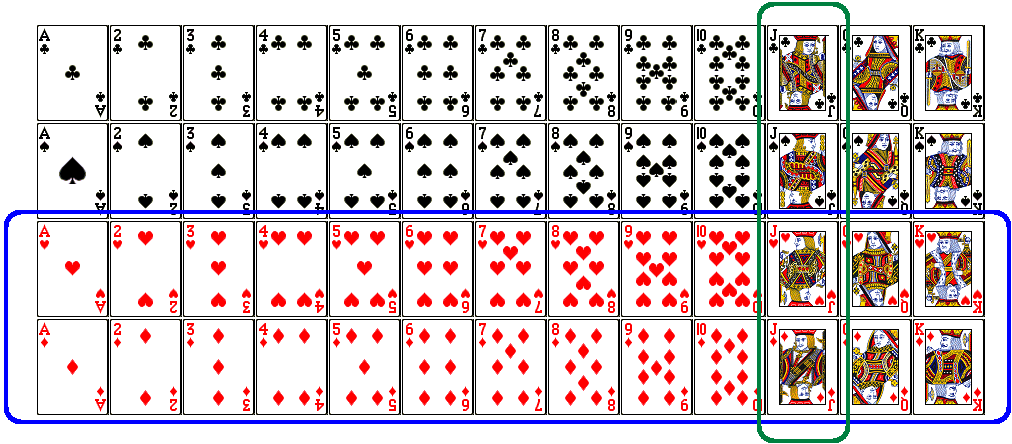
\includegraphics[width=0.7\textwidth]{3-1_define_probability/figures/cards}
\end{figure}

\vspace{-0.75cm}

\soln{\onslide<2->{
\begin{align*}
P(jack~or~red) &= P(jack) + P(red) - \orange{$P(jack~and~red)$} \\
&= \frac{4}{52} + \frac{26}{52} - \frac{2}{52} = \frac{28}{52}
\end{align*}
}}

\vfill

\ct{Figure from \webURL{http://www.milefoot.com/math/discrete/counting/cardfreq.htm}.}

\end{frame}

%%%%%%%%%%%%%%%%%%%%%%%%%%%%%%%%%%%%
\subsection{Probabilities when events are not disjoint}

%%%%%%%%%%%%%%%%%%%%%%%%%%%%%%%%%%%%

\begin{frame}
\frametitle{Practice}

\pq{What is the probability that a randomly sampled applicant is a black \underline{or} a woman in the Bertrand-Mullainathan dataset?}

{\small
\begin{center}
\begin{tabular}{l  cc c}
            & \multicolumn{2}{c}{\textit{Gender}} & \\
\cline{2-3}
\textit{Race} &Man & Woman & Total \\
\hline
Black         & 549 & 1886 & 2435 \\
White         & 575 & 1860 & 2435 \\
\hline
Total       & 1124 & 3476 & 4870
\end{tabular}
\end{center}
}


\begin{enumerate}[(a)]
\item $ 0.8 $
\solnMult{$ 0.88 $}
\item $\frac{1886}{2435}$
\item $\frac{1886}{4870}$
\end{enumerate}

\end{frame}

%%%%%%%%%%%%%%%%%%%%%%%%%%%%%%%%%%%%

\begin{frame}
\frametitle{Recap}

\formula{General addition rule}{\[ P(A~or~B) = P(A) + P(B) - P(A~and~B) \]}

\Note{For disjoint events $P(A~and~B) = 0$, so the above formula simplifies to $P(A~or~B) = P(A) + P(B)$.}

\end{frame}

%%%%%%%%%%%%%%%%%%%%%%%%%%%%%%%%%%%%
%%%%%%%%%%%%%%%%%%%%%%%%%%%%%%%%%%%%

\subsection{Probability distributions}

%%%%%%%%%%%%%%%%%%%%%%%%%%%%%%%%%%%%

\begin{frame}
\frametitle{Probability distributions}

A \hl{probability distribution} lists all possible events and the probabilities with which they occur.

\begin{itemize}
\item The probability distribution for a toss of a coin:
{\footnotesize 
\begin{center}
\begin{tabular}{r | c | c}
Event    & Head		& Tail \\
\hline
Probability	& 0.5		& 0.5 \\
\end{tabular}
\end{center}
}

\pause

\item Rules for probability distributions:
\begin{enumerate}
\item The events listed must be disjoint
\item Each probability must be between 0 and 1
\item The probabilities must total 1
\end{enumerate}

\pause

\item The probability distribution for two tosses of coin:
\soln{
\only<2->{
{\footnotesize
\begin{center}
\begin{tabular}{r | c | c | c | c}
Event		& HH 	& HT		& TH		& TT \\
\hline
Probability	& 0.25	& 0.25	& 0.25	& 0.25 \\
\end{tabular}
\end{center}
}}}

\end{itemize}

\end{frame}

%%%%%%%%%%%%%%%%%%%%%%%%%%%%%%%%%%%%

\begin{frame}
\frametitle{Practice}

\pq{In a pre-election survey, 48\% of respondents in Bihar said they will vote for the NDA. What is the probability that a randomly selected respondent from this sample is a MGB voter?}

\begin{enumerate}[(a)]
\item 0.52
\item more than 0.52
\item less than 0.52
\solnMult{cannot calculate using only the information given}
\end{enumerate}

\soln{\only<2>{\orange{If the only two coalitions are the NDA and the MGB, then (a) is possible. However it is also possible that some people do not affiliate with a political party or affiliate with a party other than these two coalitions. Then (c) is also possible. However (b) is definitely not possible since it would result in the total probability for the sample space being above 1.}}}

\end{frame}


%%%%%%%%%%%%%%%%%%%%%%%%%%%%%%%%%%%%

\subsection{Complement of an event}

%%%%%%%%%%%%%%%%%%%%%%%%%%%%%%%%%%%%

\begin{frame}
\frametitle{Sample space and complements}

\hl{Sample space} is the collection of all possible outcomes of a trial.

\begin{itemize}
\item Toss of a coin $S = \{ H, T \}$
\item Two tosses of a coin \soln{\pause{$S = \{HH,TT, HT, TH \}$}}
\end{itemize}

\pause

\hl{Complementary events} are two mutually exclusive events whose probabilities that add up to 1.

\begin{itemize}
\item If we know that the toss of a coin didn't yield head, what is the outcome?
\{ \sout{\textcolor{gray}{H}}, \orange{T} \} $\rightarrow$ head and tail are \hl{complementary} outcomes.
\item Two tosses of a coin: if we know that they are not both tails, what are the possible combinations?
\soln{\pause{\{ \orange{HH}, \sout{\textcolor{gray}{TT}}, \orange{HT}, \orange{TH} \} }}
\end{itemize}

\end{frame}

%%%%%%%%%%%%%%%%%%%%%%%%%%%%%%%%%%%%

\subsection{Independence}

%%%%%%%%%%%%%%%%%%%%%%%%%%%%%%%%%%%%

\begin{frame}
\frametitle{Independence}

Two processes are \hl{independent} if knowing the outcome of one provides no useful information about the outcome of the other.

\pause

\begin{itemize}

\item Knowing that the coin landed on a head on the first toss \underline{does not} provide any useful information for determining what the coin will land on in the second toss. $\rightarrow$ Outcomes of two tosses of a coin are independent.

\pause

\item Knowing that the first card drawn from a deck is an ace \underline{does} provide useful information for determining the probability of drawing an ace in the second draw. $\rightarrow$ Outcomes of two draws from a deck of cards (without replacement) are dependent.

\end{itemize}

\end{frame}

%%%%%%%%%%%%%%%%%%%%%%%%%%%%%%%%%%%%
\begin{frame}{Practice}
\pq{\small{Economist Priyanka Pandey surveyed a random sample of IIT-BHU students. One of the questions asked in the survey was about the perceptions of academic ability of lower-caste students. 61\% upper-caste students felt that academic ability of SC students was lower than others, whereas 46 \% SC-ST students felt the same. Which of the below is true?}}

Perception about caste and caste are most likely
\begin{enumerate}[(a)]
\item complementary
\item mutually exclusive
\item independent
\solnMult{dependent}
\item disjoint
\end{enumerate}


\Note{You can read the full article here- \ct{\webURL{https://www.epw.in/engage/article/Survey-at-an-IIT-Campus-Shows-How-Caste-Affects-Students-Perceptions}.}}

\end{frame}


%%%%%%%%%%%%%%%%%%%%%%%%%%%%%%%%%%%%
\begin{frame}
\frametitle{}

\formula{Checking for independence}{If P(A occurs, given that B is true) = $P(A~|~B) = P(A)$, then A and B are independent.}

$\:$ \\

\soln{\pause{P(demonetization curbed black money) = 0.25 \\
\pause
$\:$ \\
P(randomly selected respondent says demonetization curbed black money, given that the resident is a BJP voter) = \\ P(demonetization curbed black money $|$ BJP) = 0.45 \\
$\:$ \\
P(demonetization curbed black money $|$ Congress) = 0.15 \\
$\:$ \\
P(demonetization curbed black money $|$ Others) = 0.20 \\
$\:$ \\
\pause
P(demonetization curbed black money) varies by party-affiliation, therefore the two variables are mostly likely dependent.
}}

\end{frame}

%%%%%%%%%%%%%%%%%%%%%%%%%%%%%%%%%%%%

\begin{frame}
\frametitle{Determining dependence based on sample data}

\begin{itemize}

\item If conditional probabilities calculated based on sample data suggest dependence between two variables, the next step is to conduct a hypothesis test to determine if the observed difference between the probabilities is likely or unlikely to have happened by chance.

\item If the observed difference between the conditional probabilities is large, then there is stronger evidence that the difference is real.

\item If a sample is large, then even a small difference can provide strong evidence of a real difference.

\end{itemize}

\pause

\dq{{\small We saw that P(callback $|$ Black) = 6.4\% and P(callback $|$ White) = 9.7\%. Under which condition would you be more convinced of a real difference between the proportions of callbacks for African-American and White CVs? $n = 50$ or $n = 5,000$}} \pause \soln{$n = 5,000$}

\end{frame}

%%%%%%%%%%%%%%%%%%%%%%%%%%%%%%%%%%%%

\begin{frame}
\frametitle{}

For two independent events, the product rule is:
\begin{tcolorbox}[colback=textboxgreen, colframe=textboxred]
\begin{align*}
P(A~and~B) = P(A) \times P(B)  \\
\small{\text{Or more generally,} \;  P(A_1~and~\cdots~and~A_k) = P(A_1) \times \cdots \times P(A_k)}
\end{align*}
\end{tcolorbox}

\pause

\dq{You toss a coin twice, what is the probability of getting two tails in a row?}

\pause
\begin{tcolorbox}[colback=textboxred!75, colframe = white]
\color{white}
\[ P(\text{T on the first toss}) \times  P(\text{T on the second toss}) = \frac{1}{2} \times \frac{1}{2} = \frac{1}{4} \]
\end{tcolorbox}

\end{frame}

%%%%%%%%%%%%%%%%%%%%%%%%%%%%%%%%%%%%

\begin{frame}{Practice}

\pq{A recent survey suggests that 80.6\% of Shivaji Nagar had no saving to buy ration during the lockdown. Assuming that the saving rate stayed constant, what is the probability that two randomly selected persons from Shivaji Nagar had no savings?}

\begin{columns}
\column{0.4\textwidth}

\begin{enumerate}[(a)]
\item $80.6^2$
\solnMult{ $0.806^2$ }
\item $0.806 \times 2$
\item $(1 - 0.806)^2$
\end{enumerate}

\column{0.6\textwidth}

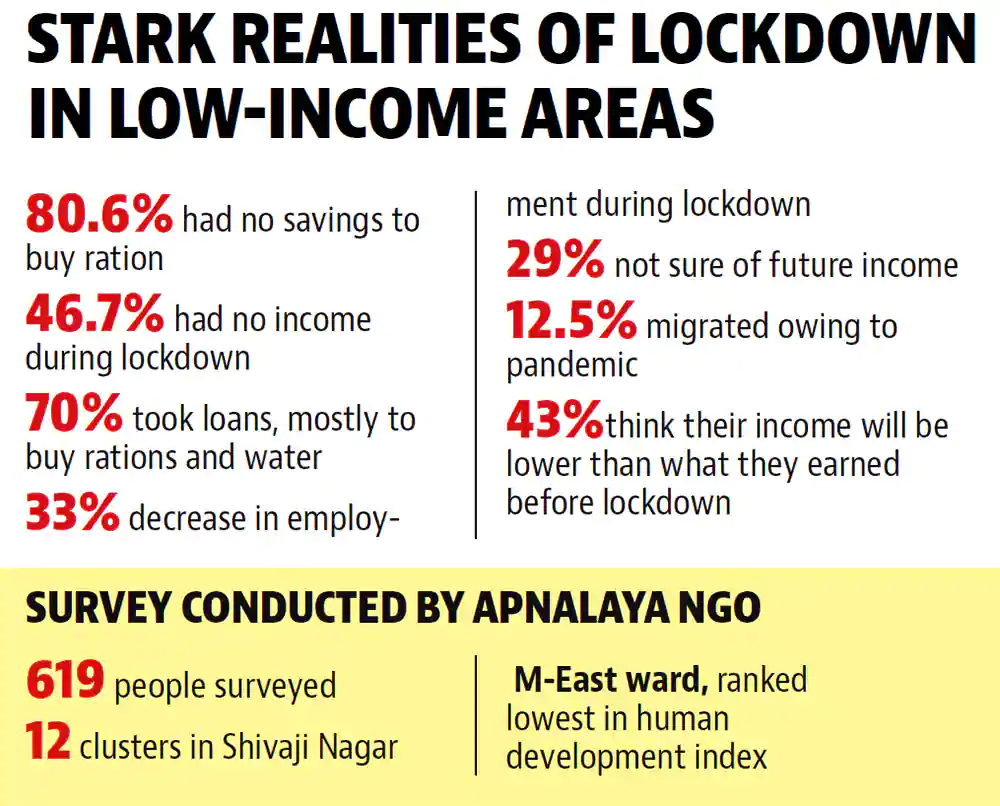
\includegraphics[width=0.6\textwidth]{graphs/l03f01.png}
\end{columns}

\ct{ \webURL{https://www.hindustantimes.com/mumbai-news/with-no-income-during-lockdown-people-in-slums-forced-to-borrow-money-for-water-survey/story-px8fdUIWQQTXbjBCJPBhlK.html}}

\end{frame}

%%%%%%%%%%%%%%%%%%%%%%%%%%%%%%%%%%%%

\begin{frame}
\frametitle{Putting everything together...}

\dq{If we were to randomly select 5 households from Shivaji Nagar, what is the probability that at least one had no saving?}

\begin{itemize}

\item If we were to randomly select 5 households, the sample space for the number of households without savings would be:
\[ S = \{0, 1, 2, 3, 4, 5\} \]

\item We are interested in instances where at least one household is without saving:
\[ S = \{0, \orange{$1, 2, 3, 4, 5$} \} \]

\item So we can divide up the sample space into two categories:
\[ S = \{0, \orange{at~least~one} \} \]

\end{itemize}

\end{frame}

%%%%%%%%%%%%%%%%%%%%%%%%%%%%%%%%%%%%
%%%%%%%%%%%%%%%%%%%%%%%%%%%%%%%%%%%%

\section{Conditional probability}

%%%%%%%%%%%%%%%%%%%%%%%%%%%%%%%%%%%%

\subsection{Exploring probabilities with a contingency table}

%%%%%%%%%%%%%%%%%%%%%%%%%%%%%%%%%%%%

\begin{frame}

\index{data!photo\_classify|(}

\newcommand{\fashN}{1822}
\newcommand{\fashYY}{197}
\newcommand{\fashYN}{22}
\newcommand{\fashYA}{219}
\newcommand{\fashNY}{112}
\newcommand{\fashNN}{1491}
\newcommand{\fashNA}{1603}
\newcommand{\fashAY}{309}
\newcommand{\fashAN}{1513}
\newcommand{\fashAA}{\fashN{}}
\newcommand{\fashCYPY}{0.96}
\newcommand{\fashCYPN}{0.04}
\newcommand{\fashCNPY}{0.07}
\newcommand{\fashCNPN}{0.93}

\begin{tcolorbox}[colback = textboxgreen!75]
Dataset : \texttt{photoclassify} \\
What it contains: 1822 photos from a photo-sharing website \\
Objective: figure out whether a photo is about fashion or not. 
Method:  \\
\begin{columns}
\column{0.5\textwidth}
 Each photo gets two classifications (the variable is called \texttt{mach\_learn}):
          \begin{itemize}
          \item[1] \texttt{predfashion}
          \item[2] \texttt{prednot}
          \end{itemize}
 \column{0.5\textwidth}
 Each photo also gets categorized (the variable is called \texttt{truth}):
          \begin{itemize}
           \item[1] \texttt{fashion}
           \item[2] \texttt{not}
           \end{itemize}
\end{columns}
\end{tcolorbox}

\pause

\begin{tcolorbox}[colback=textboxred!85, coltext=white]
\begin{center}
\begin{figure}[ht]
\centering
\small
\begin{tabular}{ll ccc rr}
&& \multicolumn{2}{c}{\texttt{truth}} & \hspace{1cm} &  \\
\cline{3-4}
&& \resp{fashion} & \resp{not} & Total  \\
\cline{2-5}
& \resp{pred\_fashion} &
    \fashYY{} & \fashYN{} & \fashYA{} \\
\raisebox{1.5ex}[0pt]{\texttt{mach\_learn}}
    & \resp{pred\_not} \hspace{0.5cm} &
    \fashNY{} & \fashNN{} & \fashNA{}   \\
\cline{2-5}
& Total & \fashAY{} & \fashAN{} & \fashN{} \\
\end{tabular}
\caption{Contingency table summarizing the
    \data{photo\_classify} data set.}
\label{contTableOfFashionPhotos}
\end{figure}
\end{center}
\end{tcolorbox}

\end{frame}

%%%%%%%%%%%%%%%%%%%%%%%%%%%%%%%%%%%%

\begin{frame}

\dq{What is the probability that a photo is not actually about fashion?}


{\small
\begin{center}
\begin{tabular}{ll ccc rr}
&& \multicolumn{2}{c}{\texttt{truth}} & \hspace{1cm} &  \\
\cline{3-4}
&& \resp{fashion} & \resp{not} & Total  \\
\cline{2-5}
& \resp{pred\_fashion} &
    197 & 22 & 219 \\
\raisebox{1.5ex}[0pt]{\texttt{mach\_learn}}
    & \resp{pred\_not} \hspace{0.5cm} &
    112 & 1491 & 1603   \\
\cline{2-5}
& Total & 309 & 1513 & 1822 \\
\end{tabular}
\end{center}
}
\end{frame}

%%%%%%%%%%%%%%%%%%%%%%%%%%%%%%%%%%%%

\subsection{Marginal and joint probabilities}

%%%%%%%%%%%%%%%%%%%%%%%%%%%%%%%%%%%%

\begin{frame}
\frametitle{Marginal probability}

\dq{What is the probability that a photo is not actually about fashion?}

{\small
\begin{center}
\begin{tabular}{ll ccc rr}
&& \multicolumn{2}{c}{\texttt{truth}} & \hspace{1cm} &  \\
\cline{3-4}
&& \resp{fashion} & \resp{not} & Total  \\
\cline{2-5}
& \resp{pred\_fashion} &
    197 & 22 & 219 \\
\raisebox{1.5ex}[0pt]{\texttt{mach\_learn}}
    & \resp{pred\_not} \hspace{0.5cm} &
    112 & 1491 & 1603   \\
\cline{2-5}
& Total & 309 & \only<1>{1513}\only<2->{\red{1513}} & \only<1>{1822}\only<2->{\red{1822}} \\
\end{tabular}
\end{center}
}

\onslide<2->{P(not fashion) = $\frac{1513}{1822} \approx 0.83$} \\

\end{frame}

%%%%%%%%%%%%%%%%%%%%%%%%%%%%%%%%%%%%

\begin{frame}
\frametitle{Joint probability}

\dq{What is the probability that a photo was about fashion and the ML method correctly classified it as one?}

{\small
\begin{center}
\begin{tabular}{ll ccc rr}
&& \multicolumn{2}{c}{\texttt{truth}} & \hspace{1cm} &  \\
\cline{3-4}
&& \resp{fashion} & \resp{not} & Total  \\
\cline{2-5}
& \resp{pred\_fashion} &
   \only<1>{197}\only<2>{\red{197}} & 22 & 219 \\
\raisebox{1.5ex}[0pt]{\texttt{mach\_learn}}
    & \resp{pred\_not} \hspace{0.5cm} &
    112 & 1491 & 1603   \\
\cline{2-5}
& Total & 309 & 1513 & \only<1>{1822}\only<2>{\red{1822}} \\
\end{tabular}
\end{center}
}

\onslide<2->{P(truth and predicted) = $\frac{197}{1822} \approx 0.11$} \\

\end{frame}

%%%%%%%%%%%%%%%%%%%%%%%%%%%%%%%%%%%%

\subsection{Defining conditional probability}

%%%%%%%%%%%%%%%%%%%%%%%%%%%%%%%%%%%%

\begin{frame}\frametitle{Conditional probability}

\begin{tcolorbox}[colback = textboxgreen!75]
The conditional probability of the outcome of interest $\textcolor{purple}{A}$ given condition $\textcolor{pink}{B}$ is calculated as
\[ P(\textcolor{purple}{A}|\textcolor{pink}{B}) = \frac{P(\textcolor{purple}{A}~and~\textcolor{pink}{B})}{P(\textcolor{pink}{B})} \]
\end{tcolorbox}

\pause

\twocol{0.5}{0.5}
{
{\small
\begin{center}
\begin{tabular}{ll ccc rr}
&& \multicolumn{2}{c}{\texttt{truth}} & \hspace{1cm} &  \\
\cline{3-4}
&& \resp{fashion} & \resp{not} & Total  \\
\cline{2-5}
& \resp{pred\_fashion} &
    197 & 22 & 219 \\
\raisebox{1.5ex}[0pt]{\texttt{mach\_learn}}
    & \resp{pred\_not} \hspace{0.5cm} &
    112 & 1491 & 1603   \\
\cline{2-5}
& Total & 309 & 1513 & 1822 \\
\end{tabular}
\end{center}
}
}
{
\begin{eqnarray*}
&&P(\textcolor{purple}{truth} | \textcolor{pink}{predicted} ) \\
&&= \frac{P(\textcolor{purple}{truth}  ~ and ~ \textcolor{pink}{predicted})}{P(\textcolor{pink}{predicted})} \\
\pause
&&= \frac{\textcolor{purple}{197} / 1822}{\textcolor{pink}{219} /1822} \\
\pause
&&= \frac{\textcolor{purple}{197}}{\textcolor{pink}{219}} \\
\pause
&&= 0.9
\end{eqnarray*}
}

\end{frame}



%%%%%%%%%%%%%%%%%%%%%%%%%%%%%%%%%%%%

\begin{frame}
\frametitle{Conditional probability (cont.)}

\dq{If we know that a particular photo is about fashion, what is the probability that the machine learning classifier correctly predicted it as one?}

{\small
\begin{center}
%\begin{tabular}{l | >{\columncolor[gray]{0.7}[0pt]}c c | c}
\begin{tabular}{l c   >{\columncolor[gray]{0.7}[0pt]} c c rr}
&& \multicolumn{2}{c}{\texttt{truth}} & \hspace{1cm} &  \\
\cline{3-4}
&& \resp{fashion} & \resp{not} & Total  \\
\cline{2-5}
& \resp{pred\_fashion} &
    197 & 22 & 219 \\
\raisebox{1.5ex}[0pt]{\texttt{mach\_learn}}
    & \resp{pred\_not} \hspace{0.5cm} &
    112 & 1491 & 1603   \\
\cline{2-5}
& Total & 309 & 1513 & 1822 \\
\end{tabular}
\end{center}
}

\pause

{
\begin{eqnarray*}
&&P(\textcolor{purple}{predicted} | \textcolor{pink}{truth} ) \\
&&= \frac{P(\textcolor{purple}{predicted}  ~ and ~ \textcolor{pink}{truth})}{P(\textcolor{pink}{truth})} \\
\pause
&&= \frac{\textcolor{purple}{197} / 1822}{\textcolor{pink}{309} /1822} \\
\pause
&&= \frac{\textcolor{purple}{197}}{\textcolor{pink}{309}} \\
\pause
&&= 0.64
\end{eqnarray*}
}


\end{frame}

%%%%%%%%%%%%%%%%%%%%%%%%%%%%%%%%%%%%

\subsection{General multiplication rule}

%%%%%%%%%%%%%%%%%%%%%%%%%%%%%%%%%%%%

\begin{frame}
\frametitle{General multiplication rule}

\begin{itemize}

\item Earlier we saw that if two events are independent, their joint probability is simply the product of their probabilities. If the events are not believed to be independent, the joint probability is calculated slightly differently.

\pause

\item If $\textcolor{purple}{A}$ and $\textcolor{pink}{B}$ represent two outcomes or events, then
\formula{\[ P(\textcolor{purple}{A}~and~\textcolor{pink}{B}) = P(\textcolor{purple}{A}|\textcolor{pink}{B}) \times P(\textcolor{pink}{B}) \]}
Note that this formula is simply the conditional probability formula, rearranged.

\pause

\item It is useful to think of $\textcolor{purple}{A}$ as the outcome of interest and $\textcolor{pink}{B}$ as the condition.

\end{itemize}

\end{frame}

%%%%%%%%%%%%%%%%%%%%%%%%%%%%%%%%%%%%

\subsection{Independence considerations in conditional probability}

%%%%%%%%%%%%%%%%%%%%%%%%%%%%%%%%%%%%

\begin{frame}
\frametitle{Independence and conditional probabilities}

Consider the following (hypothetical) distribution of gender and major of students in an introductory statistics class:

{\small
\begin{center}
\begin{tabular}{l | c c | c}
			& social	& non-social 		&  \\
			& science	& science	& total \\
\hline
female		& 30		& 20		& 50 \\
male			& 30		& 20		& 50 \\
\hline
total			& 60		& 40		& 100
\end{tabular}
\end{center}
}

\pause

\begin{itemize}

\item The probability that a randomly selected student is a social science major is \pause $\frac{60}{100} = 0.6$. 

\pause

\item The probability that a randomly selected student is a social science major given that they are female is \pause $\frac{30}{50} = 0.6$. 

\pause

\item Since $P(SS | M)$ also equals 0.6, major of students in this class does not depend on their gender: P(SS $|$ F) = P(SS).

\end{itemize}

\end{frame}

%%%%%%%%%%%%%%%%%%%%%%%%%%%%%%%%%%%%

\begin{frame}
\frametitle{Independence and conditional probabilities (cont.)}

Generically, if $P(\textcolor{purple}{A}|\textcolor{pink}{B}) = P(\textcolor{purple}{A})$ then the events $\textcolor{purple}{A}$ and $\textcolor{pink}{B}$ are said to be independent.

\pause

\begin{itemize}

\item Conceptually: Giving $\textcolor{pink}{B}$ doesn't tell us anything about $\textcolor{purple}{A}$.

\pause

\item Mathematically: We know that if events $\textcolor{purple}{A}$ and $\textcolor{pink}{B}$ are independent, $P(\textcolor{purple}{A}~and~\textcolor{pink}{B}) = P(\textcolor{purple}{A}) \times P(\textcolor{pink}{B})$. Then,
\[ P(\textcolor{purple}{A}|\textcolor{pink}{B}) = \frac{P(\textcolor{purple}{A}~and~\textcolor{pink}{B})}{P(\textcolor{pink}{B})} = \frac{P(\textcolor{purple}{A}) \times P(\textcolor{pink}{B})}{P(\textcolor{pink}{B})} = P(\textcolor{purple}{A}) \]

\end{itemize}

\end{frame}

%%%%%%%%%%%%%%%%%%%%%%%%%%%%%%%%%%%%

\subsection{Tree diagrams}

%%%%%%%%%%%%%%%%%%%%%%%%%%%%%%%%%%%%

\begin{frame}
\frametitle{Inverting probabilities}

\dq{When an applicant applies for a job, there are two possibilities: callback, and no callback. If the candidate has a Black-sounding name, what is the probability that she got a callback?}

\pause

\twocol{0.6}{0.3}{
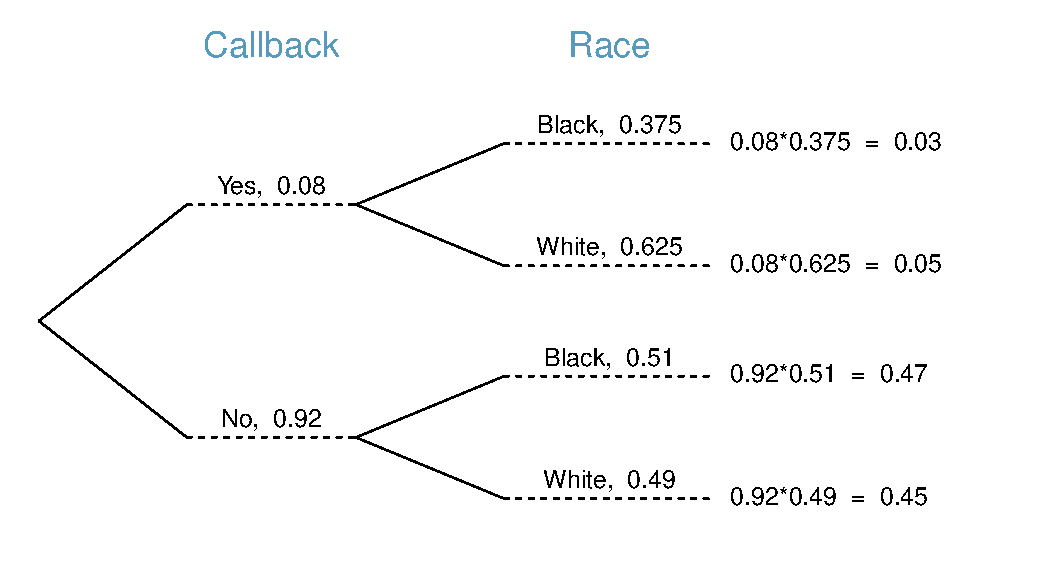
\includegraphics[width=\textwidth]{graphs/l03f02} 
}
{
\pause
{\footnotesize
\begin{eqnarray*}
&&P(\textcolor{purple}{Callback} | \textcolor{pink}{Black}) \\
\pause
&&= \frac{P(\textcolor{purple}{Callback}~and~\textcolor{pink}{Black})}{P(\textcolor{pink}{Black})} \\
\pause
&&= \frac{0.03}{0.03 + 0.047} \\
\pause
&&= 0.06
\end{eqnarray*}
}
}

\pause

\Note{Tree diagrams are useful for inverting probabilities: we are given $P(\textcolor{purple}{Black}|\textcolor{pink}{Callback})$ and asked for $P(\textcolor{purple}{Callback} | \textcolor{pink}{Black})$.}

\end{frame}

%%%%%%%%%%%%%%%%%%%%%%%%%%%%%%%%%%%

\subsection{Bayes' Theorem}

%%%%%%%%%%%%%%%%%%%%%%%%%%%%%%%%%%%%

\begin{frame}
\frametitle{Bayes' Theorem}

\begin{itemize}

\item The conditional probability formula we have seen so far is a special case of the Bayes' Theorem, which is applicable even when events have more than just two outcomes.

\pause 

\item \hl{Bayes' Theorem:}


\formula{
\begin{tcolorbox}[colback = textboxgreen!75]
\[ P(\textcolor{purple}{outcome~A_1~of~variable~1~}|\textcolor{pink}{~outcome~B~of~variable~2}) \]
\[ = \frac{P(\textcolor{pink}{B}|\textcolor{purple!95}{A_1})P(\textcolor{purple!95}{A_1})}{P(\textcolor{pink}{B}|\textcolor{purple!95}{A_1})P(\textcolor{purple!95}{A_1}) + P(\textcolor{pink}{B}|\textcolor{purple!90}{A_2})P(\textcolor{purple!90}{A_2}) + \cdots + P(\textcolor{pink}{B}|\textcolor{purple!85}{A_k})P(\textcolor{purple!85}{A_k})} \]
\end{tcolorbox}
}
where $\textcolor{purple}{A_2}$, $\cdots$, $\textcolor{purple}{A_k}$ represent all other possible outcomes of variable 1.

\end{itemize}

\end{frame}

%%%%%%%%%%%%%%%%%%%%%%%%%%%%%%%%%%%

\begin{frame}
\frametitle{Application activity: Inverting probabilities}

\app{{\footnotesize Stores Murugan, Saravana, and Nilgiris have 50, 75, and 100 employees and,
respectively, 50, 60, 70 percent of these are women. Resignations are equally likely
among all employees, regardless of sex. One employee resigns, and this happens to be a
woman. What is the probability that she works in Nilgiris store?
}}

\end{frame}

%%%%%%%%%%%%%%%%%%%%%%%%%%%%%%%%%%%

\begin{frame}
\frametitle{Application activity: Inverting probabilities (cont.)}

Start figuring out the probability of resignation from each store.
\\
\pause
$P(W_{1}|M) = 0.5$, $P(W_{2}|S) = 0.6$, $P(W_{3}|N) = 0.7$. \\
$P(M) = 2/9$, $P(S) = 1/3$, $P(N) = 4/9$. \\

\pause

\[ P(N| W_3) = \frac{P(N~and~W_3)}{P(W_3)} = \frac{0.311}{0.111 + 0.2 + 0.311} = 0.5 \]
\end{frame}

%%%%%%%%%%%%%%%%%%%%%%%%%%%%%%%%%%%%

\section{Sampling from a small population}

%%%%%%%%%%%%%%%%%%%%%%%%%%%%%%%%%%%%

\begin{frame}
\frametitle{Sampling with replacement}

When sampling \hl{with replacement}, you put back what you just drew.

\pause

\begin{itemize}

\item Imagine you have a bag with 5 red, 3 blue and 2 orange chips in it. What is the probability that the first chip you draw is blue?
\begin{center}
5 \textcolor{red}{$\CIRCLE$}~, 3 \textcolor{blue}{$\CIRCLE$}~, 2 \textcolor{orange}{$\CIRCLE$}
\end{center}

\pause

\[ Prob(1^{st} \text{ chip } \textcolor{blue}{B}) = \frac{3}{5 + 3 + 2} = \frac{3}{10} = 0.3 \]

\pause

\item Suppose you did indeed pull a blue chip in the first draw. If drawing with replacement, what is the probability of drawing a blue chip in the second draw?

\pause

\begin{center}
$1^{st}$ draw: 5 \textcolor{red}{$\CIRCLE$}~, 3 \textcolor{blue}{$\CIRCLE$}~, 2 \textcolor{orange}{$\CIRCLE$} \\

\pause

$2^{nd}$ draw: 5 \textcolor{red}{$\CIRCLE$}~, 3 \textcolor{blue}{$\CIRCLE$}~, 2 \textcolor{orange}{$\CIRCLE$}
\end{center}

\pause

\[ Prob(2^{nd} \text{ chip } \textcolor{blue}{B} | 1^{st} \text{ chip } \textcolor{blue}{B}) = \frac{3}{10} = 0.3 \]

\end{itemize}

\end{frame}

%%%%%%%%%%%%%%%%%%%%%%%%%%%%%%%%%%%%%

\begin{frame}
\frametitle{Sampling with replacement (cont.)}

\begin{itemize}

\item Suppose you actually pulled an orange chip in the first draw. If drawing with replacement, what is the probability of drawing a blue chip in the second draw?

\pause

\begin{center}
$1^{st}$ draw: 5 \textcolor{red}{$\CIRCLE$}~, 3 \textcolor{blue}{$\CIRCLE$}~, 2 \textcolor{orange}{$\CIRCLE$} \\
\pause
$2^{nd}$ draw: 5 \textcolor{red}{$\CIRCLE$}~, 3 \textcolor{blue}{$\CIRCLE$}~, 2 \textcolor{orange}{$\CIRCLE$}
\end{center}
\pause
\[ Prob(2^{nd} \text{ chip } \textcolor{blue}{B} | 1^{st} \text{ chip } \textcolor{orange}{O}) = \frac{3}{10} = 0.3 \]

\pause
\item If drawing with replacement, what is the probability of drawing two blue chips in a row?
\begin{center}

\pause
$1^{st}$ draw: 5 \textcolor{red}{$\CIRCLE$}~, 3 \textcolor{blue}{$\CIRCLE$}~, 2 \textcolor{orange}{$\CIRCLE$} \\
$2^{nd}$ draw: 5 \textcolor{red}{$\CIRCLE$}~, 3 \textcolor{blue}{$\CIRCLE$}~, 2 \textcolor{orange}{$\CIRCLE$}
\end{center}
\pause
\[ Prob(1^{st} \text{ chip } \textcolor{blue}{B}) \cdot Prob(2^{nd} \text{ chip } \textcolor{orange}{O} | 1^{st} \text{ chip } \textcolor{blue}{B}) = 0.3 \times 0.3 \]
\[ = 0.3^2 = 0.09 \]

\end{itemize}

\end{frame}

%%%%%%%%%%%%%%%%%%%%%%%%%%%%%%%%%%%%%

\begin{frame}
\frametitle{Sampling with replacement (cont.)}

\begin{itemize}

\item When drawing with replacement, probability of the second chip being blue does not depend on the color of the first chip since whatever we draw in the first draw gets put back in the bag.
\[ Prob(\textcolor{blue}{B} | \textcolor{blue}{B}) = Prob(\textcolor{blue}{B} | \textcolor{orange}{O}) \]

\item In addition, this probability is equal to the probability of drawing a blue chip in the first draw, since the composition of the bag never changes when sampling with replacement.
\[ Prob(\textcolor{blue}{B} | \textcolor{blue}{B}) = Prob(\textcolor{blue}{B}) \]

\item \hl{When drawing with replacement, draws are independent.}

\end{itemize}

\end{frame}


%%%%%%%%%%%%%%%%%%%%%%%%%%%%%%%%%%%%%

\begin{frame}
\frametitle{Sampling without replacement}

When drawing \hl{without replacement} you do not put back what you just drew.

\begin{itemize}

\pause

\item Suppose you pulled a blue chip in the first draw. If drawing without replacement, what is the probability of drawing a blue chip in the second draw?
\pause
\begin{center}
$1^{st}$ draw: 5 \textcolor{red}{$\CIRCLE$}~, 3 \textcolor{blue}{$\CIRCLE$}~, 2 \textcolor{orange}{$\CIRCLE$} \\
\pause
$2^{nd}$ draw: 5 \textcolor{red}{$\CIRCLE$}~, 2 \textcolor{blue}{$\CIRCLE$}~, 2 \textcolor{orange}{$\CIRCLE$}
\end{center}
\pause
\[ Prob(2^{nd} \text{ chip } \textcolor{blue}{B} | 1^{st} \text{ chip } \textcolor{blue}{B}) = \frac{2}{9} = 0.22 \]

\pause

\item If drawing without replacement, what is the probability of drawing two blue chips in a row?
\begin{center}

\pause
$1^{st}$ draw: 5 \textcolor{red}{$\CIRCLE$}~, 3 \textcolor{blue}{$\CIRCLE$}~, 2 \textcolor{orange}{$\CIRCLE$} \\
$2^{nd}$ draw: 5 \textcolor{red}{$\CIRCLE$}~, 2 \textcolor{blue}{$\CIRCLE$}~, 2 \textcolor{orange}{$\CIRCLE$}
\end{center}
\pause
\[ Prob(1^{st} \text{ chip } \textcolor{blue}{B}) \cdot Prob(2^{nd} \text{ chip } \textcolor{blue}{B} | 1^{st} \text{ chip } \textcolor{blue}{B})  = 0.3 \times 0.22 \]
\[ = 0.066 \]

\end{itemize}

\end{frame}

%%%%%%%%%%%%%%%%%%%%%%%%%%%%%%%%%%%%%

\begin{frame}
\frametitle{Sampling without replacement (cont.)}

\begin{itemize}

\item When drawing without replacement, the probability of the second chip being blue given the first was blue is not equal to the probability of drawing a blue chip in the first draw since the composition of the bag changes with the outcome of the first draw.
\[ Prob(\textcolor{blue}{B} | \textcolor{blue}{B}) \ne Prob(\textcolor{blue}{B}) \]

\pause

\item \hl{When drawing without replacement, draws are not independent.}

\pause

\item This is especially important to take note of when the sample sizes are small. If we were dealing with, say, 10,000 chips in a (giant) bag, taking out one chip of any color would not have as big an impact on the probabilities in the second draw.

\end{itemize}

\end{frame}

%%%%%%%%%%%%%%%%%%%%%%%%%%%%%%%%%%%%%

\begin{frame}
\frametitle{Practice}

\pq{In most card games cards are dealt without replacement. What is the probability of being dealt an ace and then a 3? Choose the closest answer.}

\twocol{0.3}{0.6}{
\begin{enumerate}[(a)]
\item 0.0045
\item 0.0059
\solnMult{0.0060}
\item 0.1553
\end{enumerate}
}
{
\soln{
\pause
\[ P(ace~then~3) = \frac{4}{52} \times \frac{4}{51} \approx 0.0060 \]
}}

\end{frame}

%%%%%%%%%%%%%%%%%%%%%%%%%%%%%%%%%%%%%

%%%%%%%%%%%%%%%%%%%%%%%%%%%%%%%%%%%%

\section{Random variables}

%%%%%%%%%%%%%%%%%%%%%%%%%%%%%%%%%%%%

\begin{frame}
\frametitle{Random variables}

\begin{itemize}

\item A \hl{random variable} is a numeric quantity whose value depends on the outcome of a random event
\begin{itemize}
\item We use a capital letter, like $X$, to denote a random variable
\item The values of a random variable are denoted with a lowercase letter, in this case $x$
\item For example, $P(X = x)$
\end{itemize}

\item There are two types of random variables:
\begin{itemize}
\item \hl{Discrete random variables} often take only integer values
\begin{itemize}
\item Example: Number of credit hours, Difference in number of credit hours this term vs last
\end{itemize}
\item \hl{Continuous random variables} take real (decimal) values
\begin{itemize}
\item Example: Cost of books this term, Difference in cost of books this term vs last
\end{itemize}
\end{itemize}

\end{itemize}

\end{frame}

%%%%%%%%%%%%%%%%%%%%%%%%%%%%%%%%%%%%

\subsection{Expectation}

%%%%%%%%%%%%%%%%%%%%%%%%%%%%%%%%%%%%

\begin{frame}
\frametitle{Expectation}

\begin{itemize}

\item We are often interested in the average outcome of a random variable.

\item We call this the \textcolor{hlblue}{\textit{expected value}} (mean), \\
and it is a weighted average of the possible outcomes
\formula{
\begin{tcolorbox}[colback = textboxgreen!75]
\color{denim}
\[\mu = E(X) = \sum_{i = 1}^k x_i ~ P(X = x_i)\]
\end{tcolorbox}}

\end{itemize}

\end{frame}

%%%%%%%%%%%%%%%%%%%%%%%%%%%%%%%%%%%%

\begin{frame}
\frametitle{Expected value of a discrete random variable}

\dq{In a game of cards you win \rupee 10 if you draw a heart, \rupee 50 if you draw an ace (including the ace of hearts), \rupee 100 if you draw the king of spades and nothing for any other card you draw. Write the probability model for your winnings, and calculate your expected winning.}

\pause

\begin{center}
\renewcommand{\arraystretch}{1.5}
\begin{tabular}{l | c | c | c }
Event		& $X$ 		& $P(X)$        		& $X \cdot P(X)$ \\
\hline
Heart (not ace)	& $10$		& $\frac{12}{52}$	& $10\times\frac{12}{52}$ \\
Ace			& $50$		& $\frac{4}{52}$	& $50\times\frac{4}{52}$ \\	
King of spades	& $100$		& $\frac{1}{52}$	& $100\times\frac{1}{52}$ \\	
All else		& $0$		& $\frac{35}{52}$	& $0$ \\
\hline
Total			&			&				& $E(X) = \frac{420}{52} \approx 8.1$
\end{tabular}

\end{center}

\end{frame}

%%%%%%%%%%%%%%%%%%%%%%%%%%%%%%%%%%%%

\begin{frame}
\frametitle{Expected value of a discrete random variable (cont.)}

Below is a visual representation of the probability distribution of winnings from this game:

\begin{center}
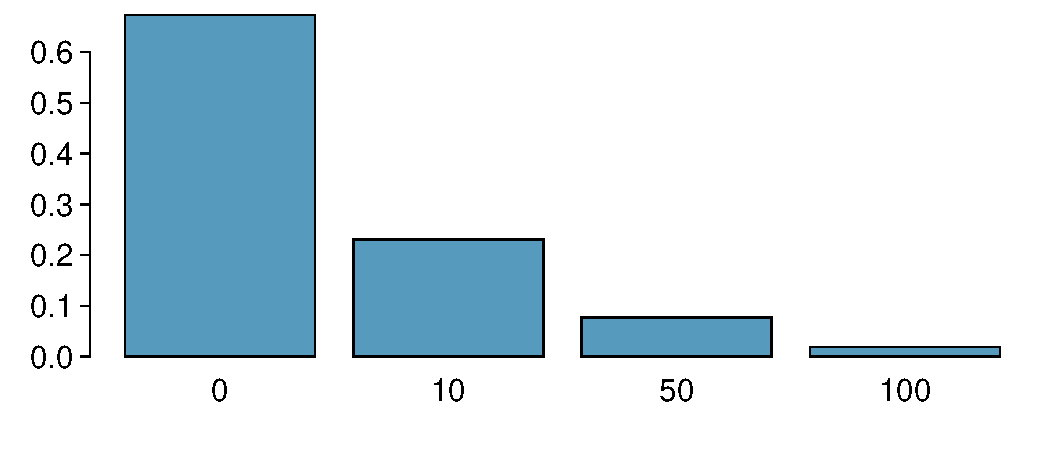
\includegraphics[width=0.8\textwidth]{graphs/l03f07}
\end{center}

\end{frame}

%%%%%%%%%%%%%%%%%%%%%%%%%%%%%%%%%%%%

\subsection{Variability in random variables}

%%%%%%%%%%%%%%%%%%%%%%%%%%%%%%%%%%%%

\begin{frame}
\frametitle{Variability}

We are also often interested in the variability in the values of a random variable.

\formula{
\[ \sigma^2 = Var(X) = \sum_{i = 1}^k (x_i - E(X))^2 P(X = x_i) \]
\[ \sigma = SD(X) = \sqrt{Var(X)} \]
}

\end{frame}

%%%%%%%%%%%%%%%%%%%%%%%%%%%%%%%%%%%%

\begin{frame}
\frametitle{Variability of a discrete random variable}

\dq{For the previous card game example, how much would you expect the winnings to vary from game to game?}

\vspace{2mm}
\only<2->{
{\footnotesize
\begin{center}
\renewcommand{\arraystretch}{2}
\begin{tabular}{c | c | c | l | p{4cm}}
  \toprule
$X$ & $P(X)$         & $X ~ P(X)$      & \multicolumn{1}{c|}{$(X - E(X))^2$}  & \multicolumn{1}{c}{$P(X) ~ (X - E(X))^2$}  \\
   \midrule  
 10 & 0.23 & 2.31 & 900.00 & 207.69 \\ 
   50 & 0.08 & 3.85 & 100.00 & 7.69 \\ 
   100 & 0.02 & 1.92 & 3600.00 & 69.23 \\ 
  0 & 0.67 & 0.00 & 1600.00 & 1076.92 \\ 
  \midrule
   &       & $E(X) = 0.81$ & & \soln{\only<3->{$V(X) = 1361.5$}} \\
 &       &                                                         & & \soln{\only<4>{$SD(X) = \sqrt{1361.5} = 36.9 $}} \\
   \bottomrule
\end{tabular}
\end{center}
}
}
\end{frame}

%%%%%%%%%%%%%%%%%%%%%%%%%%%%%%%%%%%%

\subsection{Linear combinations of random variables}

%%%%%%%%%%%%%%%%%%%%%%%%%%%%%%%%%%%%

\begin{frame}
\frametitle{Linear combinations}

\begin{itemize}

\item A \hl{linear combination} of random variables $X$ and $Y$ is given by

\[ aX + bY \]

where $a$ and $b$ are some fixed numbers.

\pause

\item The average value of a linear combination of random variables is given by
\formula{\[ E(aX + bY) = a \times E(X) + b \times E(Y) \]}

\end{itemize}

\end{frame}

%%%%%%%%%%%%%%%%%%%%%%%%%%%%%%%%%%%%

\begin{frame}
\frametitle{Calculating the expectation of a linear combination}

\dq{On average you take 10 minutes for each statistics homework problem and 15 minutes for each economics homework problem. This week you have 5 statistics and 4 economics homework problems assigned. What is the total time you expect to spend on statistics and economics homework for the week?}

\soln{
\pause
\begin{align*} 
E(S + S + S + S + S + Ec + Ec + Ec + Ec) &= 5 \times E(S) + 4 \times E(Ec) \\
&= 5 \times 10 + 4 \times 15 \\
&= 50 + 60 \\
&= 110~min 
\end{align*}
}

\end{frame}

%%%%%%%%%%%%%%%%%%%%%%%%%%%%%%%%%%%%

\subsection{Variability in linear combinations of random variables}

%%%%%%%%%%%%%%%%%%%%%%%%%%%%%%%%%%%%

\begin{frame}
\frametitle{Linear combinations}

\begin{itemize}

\item The variability of a linear combination of two independent random variables is calculated as
\formula{\[ V(aX + bY) = a^2 \times V(X) + b^2 \times V(Y) \]}

\pause 

\item The standard deviation of the linear combination is the square root of the variance.

\end{itemize}

\pause 
\vfill

\Note{If the random variables are not independent, the variance calculation gets a little more complicated and is beyond the scope of this course.}

\end{frame}

%%%%%%%%%%%%%%%%%%%%%%%%%%%%%%%%%%%%

\begin{frame}
\frametitle{Calculating the variance of a linear combination}

\dq{The standard deviation of the time you take for each statistics homework problem is 1.5 minutes, and it is 2 minutes for each economics problem. What is the standard deviation of the time you expect to spend on statistics and economics homework for the week if you have 2 statistics and 2 economics homework problems assigned? Suppose that the time it takes to complete each problem is independent of another.}

\soln{
\pause
\begin{align*} 
V(S + S + E + E) &= V(S) + V(S) + V(E) + V(E) \\
&= 2\times(V(S) +  V(E)) \\
&= 2 \times(1.5^2 + 2^2) \\
&= 12.5
\end{align*}
}

\end{frame}

%%%%%%%%%%%%%%%%%%%%%%%%%%%%%%%%%%%%

\subsection{Recap}

%%%%%%%%%%%%%%%%%%%%%%%%%%%%%%%%%%%%

\begin{frame}
\frametitle{Practice}

\pq{A casino game costs \$5 to play. If the first card you draw is red, then you get to draw a second card (without replacement). If the second card is the ace of clubs, you win \$500. If not, you don't win anything, i.e. lose your \$5. What is your expected profits/losses from playing this game? {\small Remember: profit/loss = winnings - cost.}}

\begin{multicols}{2}
\begin{enumerate}[(a)]
\item A profit of 5\textcent
\solnMult{A loss of 10\textcent}
\item A loss of 25\textcent
\item A loss of 30\textcent
\end{enumerate}
\end{multicols}

\soln{
\only<2>{
{\small
\renewcommand\arraystretch{1.25}
\begin{tabular}{l c c c r}
Event				& Win	& Profit: $X$	& $P(X)$	& $ X \times P(X)$	\\
\hline
\orange{Red}, {A}{$\clubsuit$}		& 500		& 500 - 5 = 495	& $\frac{26}{52} \times \frac{1}{51} = 	0.0098$ & 	 $495 \times 0.0098 = 4.851$ \\
Other	& 0 			& 0 - 5 = -5	& $1 - 0.0098 = 0.9902$ & $-5 \times 0.9902 = -4.951$ \\  
\hline
					&			&			& 			& $E(X) = -0.1$
\end{tabular}
}
}
}

\end{frame}

%%%%%%%%%%%%%%%%%%%%%%%%%%%%%%%%%%%%

\begin{frame}
\frametitle{Fair game}

A \hl{fair} game is defined as a game that costs as much as its expected payout, i.e. expected profit is 0.

\pause

$\:$

\dq{Do you think casino games in Vegas cost more or less than their expected payouts?}

\soln{
\pause
\begin{columns}[c]
\column{0.6\textwidth}
If those games cost less than their expected payouts, it would mean that the casinos would be losing money on average, and hence they wouldn't be able to pay for all this:
\column{0.4\textwidth}
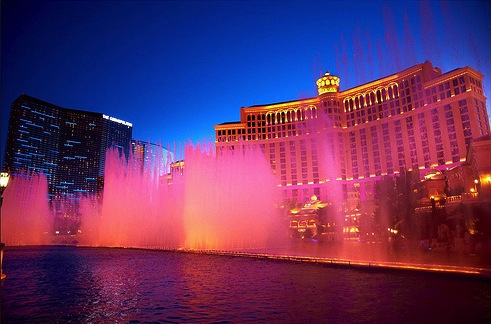
\includegraphics[width=\textwidth]{3-4_random_variables/figures/bellagio.jpg}
\end{columns}
\ct{Image by Moyan\_Brenn on Flickr \webURL{http://www.flickr.com/photos/aigle\_dore/5951714693}.}
}


\end{frame}

%%%%%%%%%%%%%%%%%%%%%%%%%%%%%%%%%%%%%

\begin{frame}
\frametitle{Simplifying random variables}

Random variables do not work like normal algebraic variables:
\[ X + X \ne 2X \]

\pause

{\small
\twocol{0.45}{0.45}
{
\begin{align*}
E(X + X) &= E(X) + E(X) \\
&= 2 E(X) \\
&~  \\
E(2X) &= 2 E(X) \\
&~ 
\end{align*}
}
{
\begin{align*}
Var(X + X) &= Var(X) + Var(X)~{\scriptsize \text{(assuming independence)}} \\
&= 2~Var(X) \\
&~  \\
Var(2X) &= 2^2~Var(X) \\
&= 4~Var(X)
\end{align*}
}
}


\pause

\vspace{3mm}

\mathhl{E(X + X)  = E(2X)}, but \mathhl{Var(X + X) \ne Var(2X)}.

\end{frame}

%%%%%%%%%%%%%%%%%%%%%%%%%%%%%%%%%%%%%

\begin{frame}
\frametitle{Adding or multiplying?}

\dq{A university in Sri City has 5 cars for transportation on campus. Historical data show that annual maintenance cost for each car is on average \rupee 10,000 with a standard deviation of \rupee 100. What is the mean and the standard deviation of the total annual maintenance cost for these vehicles?}

\pause

Note that we have 5 cars each with the given annual maintenance cost $(X_1 + X_2 + X_3 + X_4 + X_5)$, not one car that had 5 times the given annual maintenance cost $(5X)$.

\pause

{\small
\begin{eqnarray*} 
E(X_1 + X_2 + X_3 + X_4 + X_5) &=& E(X_1) + E(X_2) + E(X_3) + E(X_4) + E(X_5) \\
\pause
&=& 5 \times E(X) = 5 \times 10,000 = \text{\rupee} 50,000 \\
\pause
Var(X_1 + X_2 + X_3 + X_4 + X_5) &=& Var(X_1) + Var(X_2) + Var(X_3) + Var(X_4) + Var(X_5) \\
\pause
&=& 5 \times V(X) = 5 \times 100^2 = \text{\rupee} 50,000 \\
\pause
SD(X_1 + X_2 + X_3 + X_4 + X_5) &=& \sqrt{50,000} =  223.6
\end{eqnarray*}
}

\end{frame}


%%%%%%%%%%%%%%%%%%%%%%%%%%%%%%%%%%%%

\section{Continuous distributions}

%%%%%%%%%%%%%%%%%%%%%%%%%%%%%%%%%%%%

\begin{frame}
\frametitle{Continuous distributions}

\begin{itemize}

\item Below is a histogram of the distribution of the variable \texttt{hwy} from the dataset \texttt{mpg}. 

\item The proportion of data that falls in the shaded bins gives the probability that a randomly sampled car mileage is between 20 and 30 miles per gallon.

\end{itemize}

\begin{center}
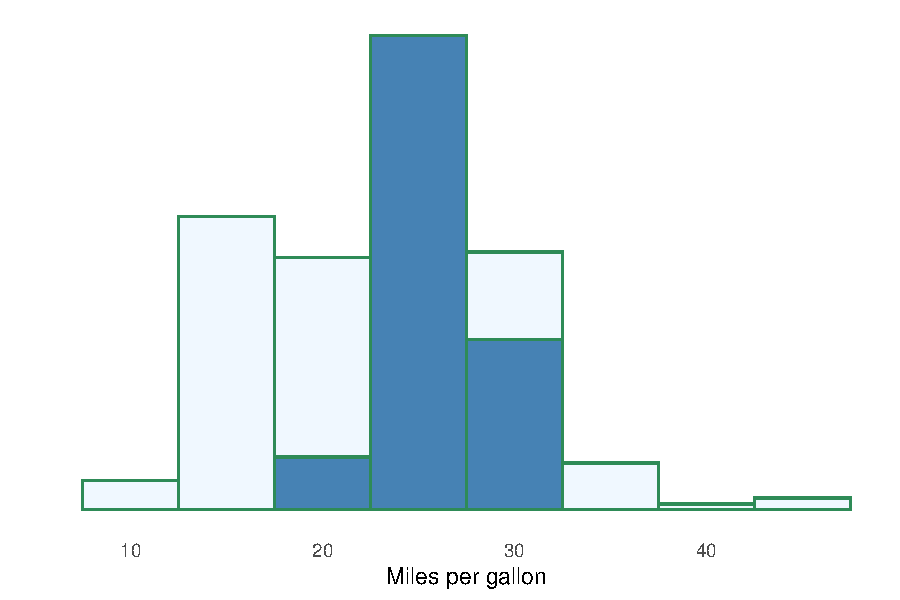
\includegraphics[width=0.65\textwidth]{graphs/l03f03}
\end{center}


\end{frame}

%%%%%%%%%%%%%%%%%%%%%%%%%%%%%%%%%%%%

\subsection{From histograms to continuous distributions}

\begin{frame}
\frametitle{From histograms to continuous distributions}

Since miles per gallon is a continuous numerical variable, its \hl{probability density function} is a smooth curve.

\begin{center}
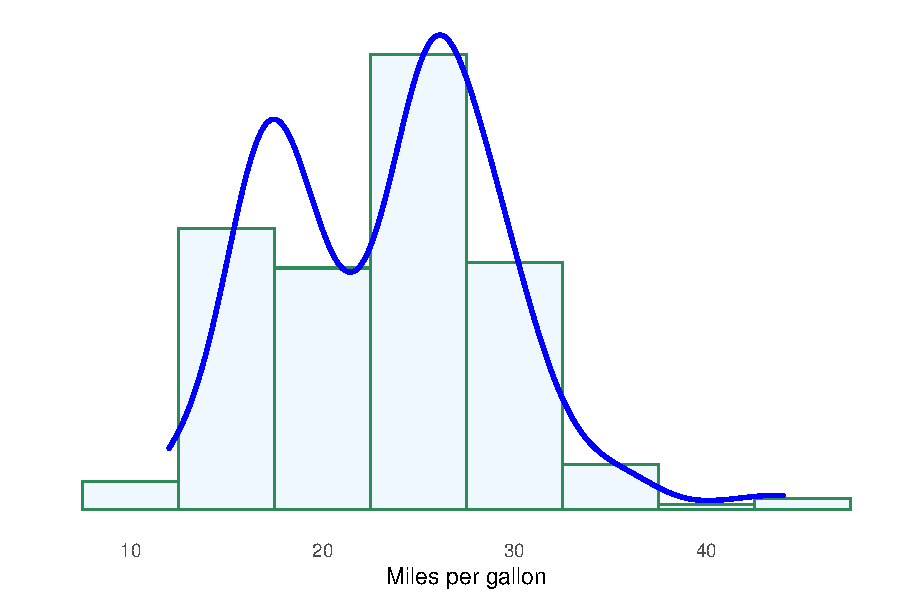
\includegraphics[width=0.65\textwidth]{graphs/l03f04}
\end{center}

\end{frame}

%%%%%%%%%%%%%%%%%%%%%%%%%%%%%%%%%%%%

\subsection{Probabilities from continuous distributions}

\begin{frame}
\frametitle{Probabilities from continuous distributions}

Therefore, the probability that a randomly sampled car has mileage between 20 mpg and 30 mpg can also be estimated as the shaded area under the curve.

\begin{center}
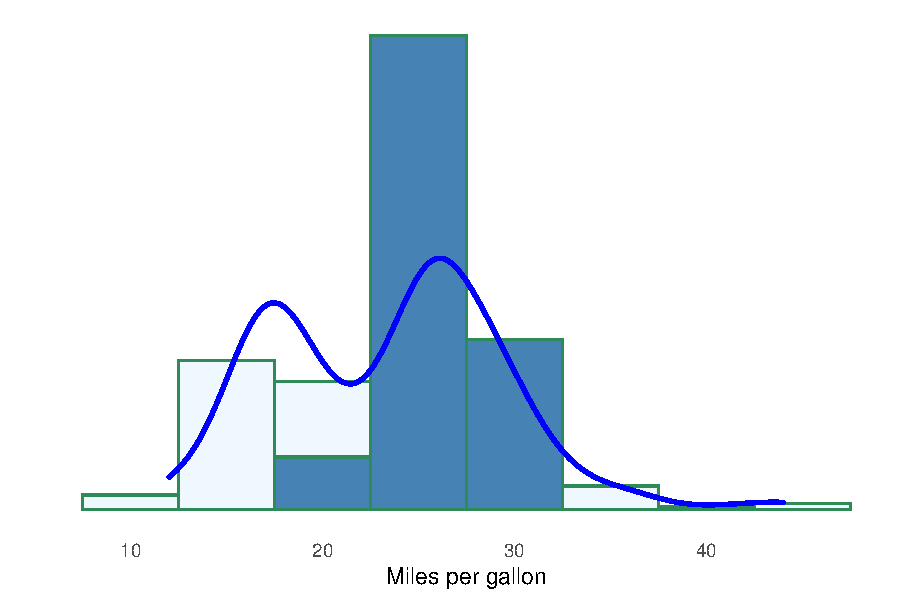
\includegraphics[width=0.65\textwidth]{graphs/l03f05}
\end{center}


\end{frame}

%%%%%%%%%%%%%%%%%%%%%%%%%%%%%%%%%%%%

\begin{frame}
\frametitle{By definition...}

Since continuous probabilities are estimated as ``the area under the curve", the probability of a car having a mileage of exactly 25 mpg (or any exact value) is defined as 0.

\begin{center}
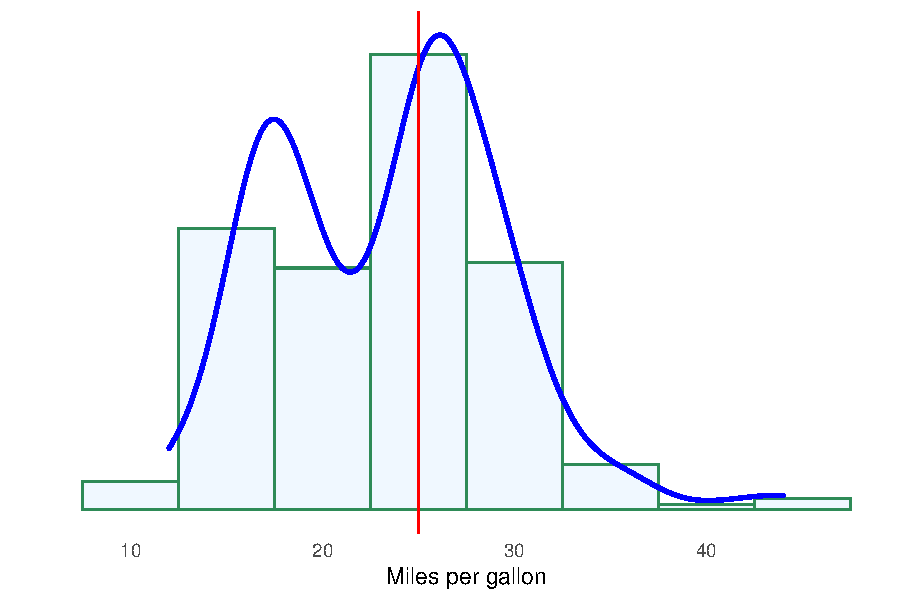
\includegraphics[width=0.65\textwidth]{graphs/l03f06}
\end{center}

\end{frame}

%%%%%%%%%%%%%%%%%%%%%%%%%%%%%%%%%%%%



\end{document}